
General equation of circle is ${\vec{x}^T\vec{x}} + 2\vec{u}^T\vec{x} $+ f = 0\\
Taking equation of the first curve to be,
\begin{align}
\norm{\vec{x}-\myvec{1\\0}}^2&=1^2\\
{\vec{x}^{T}\vec{x}+2\vec{u_1}^T\vec{x}}&=0 \label{eq:solutions/1/10/2.2.2}\\
\vec{u_1}&=\myvec{-1\\0}\\
f_1&=0\\
\vec{O_1}&=\myvec{1\\0}
\end{align}
Taking equation of the second curve to be,
\begin{align}
\norm{\vec{x}}^2 + 2\vec{u}_2^T\vec{x} + f_2&= 0\label{eq:solutions/1/10/2.1.1}\\
{\vec{x}^{T}\vec{x}}-1&=0 \label{eq:solutions/1/10/2.1.2}\\
\vec{u_2}&=\myvec{0\\0}\\
f_2&=-1\\
\vec{O_2}&=\myvec{0\\0}
\end{align}
Now, subtracting equation \eqref{eq:solutions/1/10/2.2.2} from \eqref{eq:solutions/1/10/2.1.2} We get,
\begin{align}
\vec{x}^T\vec{x}+2\vec{u_1}^T\vec{x}-\vec{x}^{T}\vec{x}-f_2&=0\\
2\vec{u}^{T}\vec{x}&=-1\\
\myvec{-2&0}\vec{x}&=-1
\end{align}
which can be written as:-
\begin{align}
\myvec{1&0}\vec{x}&=1/2 \\
\vec{x}&=\myvec{1/2 \\ 0} + \lambda \myvec{0\\1} \\
\vec{x}&=\vec{q}+\lambda\vec{m}\label{eq:solutions/1/10/2.2.10} \\
\vec{q}&=\myvec{1/2 \\ 0} \\
\vec{m}&=\myvec{0\\1}
\end{align}
Substituting \eqref{eq:solutions/1/10/2.2.10} in \eqref{eq:solutions/1/10/2.1.1}
\begin{align}
\norm{\vec{x}}^2 + 2\vec{u}_2^T\vec{x} + f_2&= 0 \\
\norm{\vec{q}+\lambda\vec{m}}^2 + f_2&= 0 \\
(\vec{q}+\lambda \vec{m})^T(\vec{q}+\lambda \vec{m})+f_2&= 0 \\
\vec{q}^T(\vec{q}+\lambda \vec{m})+\lambda  \vec{m}^T(\vec{q}+\lambda \vec{m})+f_2&= 0 \\ \norm{\vec{q}}^2+\lambda\vec{q}^T\vec{m}+\lambda\vec{m}^T\vec{q}+\lambda^2\norm{\vec{m}}^2+f_2&= 0 \\
\norm{\vec{q}}^2+2\lambda\vec{q}^T\vec{m}+\lambda^2\norm{\vec{m}}^2+f_2&= 0 
\end{align}
Taking $\lambda$ as common :
\begin{align}
\lambda(\lambda\norm{\vec{m}}^2+2\vec{q}^T\vec{m})&= -f_2-\norm{\vec{q}}^2\\
\lambda^2\norm{\vec{m}}^2&= -f_2-\norm{\vec{q}}^2\\
\lambda^2&= \frac{-f_2-\norm{\vec{q}}^2}{\norm{\vec{m}}^2} \\
\lambda^2&= \frac{3}{4} \\
\lambda&= +\sqrt{\frac{3}{4}},-\sqrt{\frac{3}{4}} \\
\lambda&= +\frac{\sqrt{3}}{2},-\frac{\sqrt{3}}{2} 
\end{align}
Substituting the value of $\lambda$ in \eqref{eq:solutions/1/10/2.2.10}
\begin{align}
\vec{x}&= \vec{q}+\lambda\vec{m} \\
\vec{A}&= \myvec{\frac{1}{2} \\ \frac{\sqrt{3}}{2}} \\
\vec{B}&= \myvec{\frac{1}{2} \\ -\frac{\sqrt{3}}{2}}
\end{align} 
Now finding the direction vector $ \vec{m}_{O_1A}$,$\
\vec{m}_{O_1B}$,$ \vec{m}_{O_2A}$ and $\ \vec{m}_{O_2B}$.
\begin{align}
\vec{m}_{O_1A}=\myvec{1\\0}-\myvec{\frac{1}{2} \\ \frac{\sqrt{3}}{2}}&=\myvec{\frac{1}{2}\\-\frac{\sqrt{3}}{2}}\\
\vec{m}_{O_1B}=\myvec{1\\0}-\myvec{\frac{1}{2} \\ -\frac{\sqrt{3}}{2}}&=\myvec{\frac{1}{2}\\\frac{\sqrt{3}}{2}}\\
\vec{m}_{O_2A}=\myvec{0\\0}-\myvec{\frac{1}{2} \\ \frac{\sqrt{3}}{2}}&=\myvec{-\frac{1}{2}\\-\frac{\sqrt{3}}{2}}\\
\vec{m}_{O_2B}=\myvec{0\\0}-\myvec{\frac{1}{2} \\ -\frac{\sqrt{3}}{2}}&=\myvec{-\frac{1}{2}\\\frac{\sqrt{3}}{2}}
\end{align}
Now finding the angle $\angle{O_1AB}$.
\begin{align}
\vec{m}_{O_1A}^T \vec{m}_{O_1B}&=\norm{ \vec{m}_{O_1A}}\norm{\vec{m}_{O_1B}}\cos\theta_1\\
\frac{\vec{m}_{O_1A}^T \vec{m}_{O_1B}}{\norm{ \vec{m}_{O_1A}}\norm{\vec{m}_{O_1B}}}&=\cos\theta_1\\
\frac{-2}{4}&=\cos\theta_1\\
\frac{-1}{2}&=\cos\theta_1\\
\theta_1&=120^{\circ}
\end{align}
Now finding the angle $\angle{O_2AB}$.
\begin{align}
\vec{m}_{O_2A}^T \vec{m}_{O_2B}&=\norm{ \vec{m}_{O_2A}}\norm{\vec{m}_{O_2B}}\cos\theta_2\\
\frac{\vec{m}_{O_2A}^T \vec{m}_{O_2B}}{\norm{ \vec{m}_{O_2A}}\norm{\vec{m}_{O_2B}}}&=\cos\theta_2\\
\frac{-2}{4}&=\cos\theta_2\\
\frac{-1}{2}&=\cos\theta_2\\
\theta_2&=120^{\circ}
\end{align}
Finding area of $\bf{O_1AB}$ and $\bf{O_2AB}$.
 \begin{align}
A_{O_1AB}=\frac{\pi\theta_1}{360}r^2-\frac{1}{2}2\sqrt{3}\\
=\frac{120}{360}\pi-\frac{1}{2}2\sqrt{3}\\
A_{O_2AB}=\frac{\pi\theta_2}{360}r^2-\frac{1}{2}2\sqrt{3}\\
=\frac{120}{360}\pi-\frac{1}{2}2\sqrt{3}
\end{align}
Area of  $\bf{O_1AO_2B}$
\begin{align}
A_{O_1AO_2B}=\frac{120}{360}\pi-\frac{1}{2}2\sqrt{3}+\frac{120}{360}\pi-\frac{1}{2}2\sqrt{3}\\
=\frac{2\pi}{3}-2\sqrt{3}
\end{align}
\begin{figure}[h!]
\centering
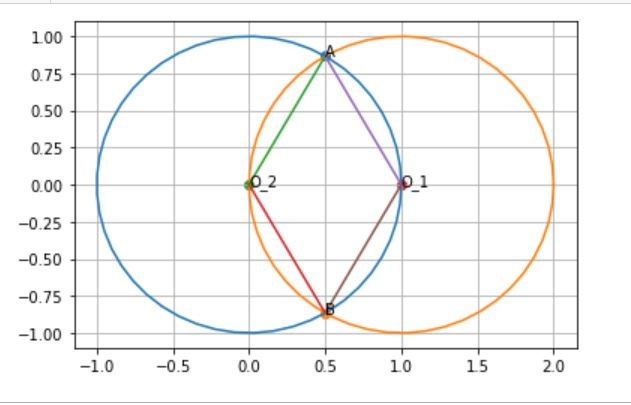
\includegraphics[width=\columnwidth]{./solutions/1/10/assignment4.JPG}
\caption{Figure depicting intersection points of circle}
\label{eq:solutions/1/10/myfig}
\end{figure}
